\documentclass[]{article}

\usepackage{geometry}
\geometry{textwidth = 18cm,textheight = 24cm}

\usepackage{multicol}
\usepackage{cite}
\usepackage{caption}
\usepackage{graphicx}
\usepackage{amsmath}
\usepackage{amssymb}
\usepackage{textcomp}
\usepackage{lmodern}
\usepackage{authblk}

\newcommand{\onlinecite}[1]{\hspace{-1 ex} \nocite{#1}\citenum{#1}} 

\begin{document}
    
\begin{center}
\LARGE{Phenomenological modeling of loop neurons}\\ 
\vspace{0.3em}
\large From: Jeffrey M. Shainline To: Andrew Dienstfrey\\
\vspace{0.0em}
\textit{\small National Institute of Standards and Technology, Boulder, CO, 80305}\\
\vspace{0.3em}
\small \today

\begin{abstract}

\vspace{1em}
\end{abstract}

\end{center}

\begin{multicols}{2}

\setcounter{tocdepth}{4}
\setcounter{secnumdepth}{4}
\tableofcontents

\section{\label{sec:introduction}Introduction}

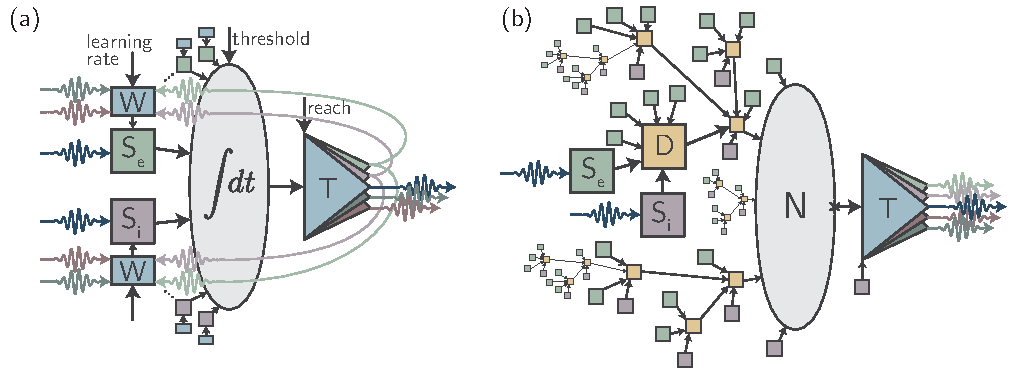
\includegraphics[width=8.6cm]{_01__schematic.pdf}
\captionof{figure}{\label{fig:schematic}Schematic of loop neuron.}

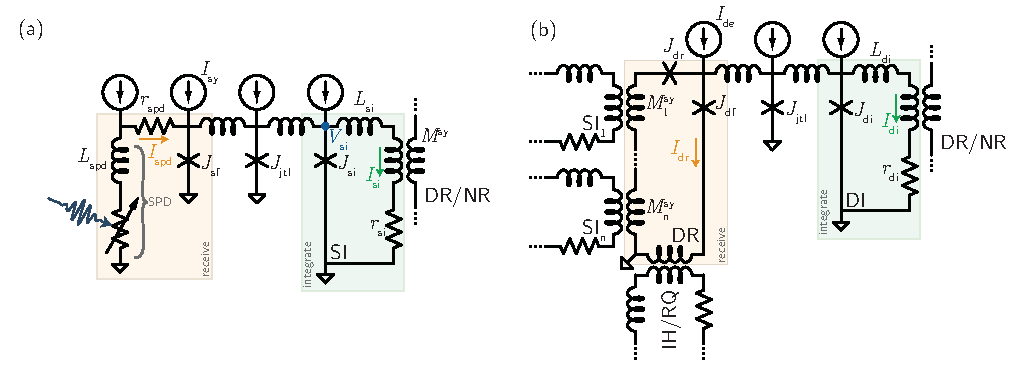
\includegraphics[width=8.6cm]{_02__circuits.pdf}
\captionof{figure}{\label{fig:circuits}Circuit diagrams of synapses and dendrites.}

\cite{sh2019_jap}

\section{\label{sec:spike_response_model}The Spike Response Model}
The spike response model (SRM) is a phenomenological model of neuron behavior that is complimentary to integrate-and-fire models. The approach leverages closed-form expressions for the response of the membrane potential to synaptic activity and production of action potentials. We can construct similar models based on loop neuron circuits to facilitate numerical analysis of loop neurons and networks.

I have only learned about SRM from the textbook called Spiking Neuron Models by Gerstner and Kistler \cite{geki2002}. From Gerstner and Kistler, pg. 102, the SRM is structured as follows. The state of neuron $i$ at time $t$ is described by a single variable, $u_i(t)$. In the absence of spikes, $u_i(t) = u_{\mathrm{rest}}$. The function
\begin{equation}
\label{eq:synaptic_response_kernel}
\epsilon_{ij}(t-t_j^{(f)})
\end{equation}
describes the time course of the response to an incoming spike train. The function $\epsilon$ is referred to as the \textit{synaptic response kernel}, and $t_j^{(f)}$. If $u_i(t)$ reaches threshold $\theta$, an output spike is triggered. The response of the variable $u_i(t)$ to the production of this action potential is modeled by the function
\begin{equation}
\label{eq:reset_kernel}
\eta(t-\hat{t}_i),
\end{equation}
where $\hat{t}_i$ is the time of the last action potential produced by neuron $i$. The function $\eta$ is referred to as the \textit{reset kernel}. After firing, the evolution of $u_i(t)$ follows
\begin{equation}
\label{eq:spike_response_model}
u_i(t) = \eta(t-\hat{t}_i)+\sum_j w_{ij}\sum_f \epsilon_{ij}(t-t_j^{(f)}
\end{equation}


\bibliographystyle{unsrt}
\bibliography{phenomenological_modeling}

\end{multicols}

\end{document}